
% 1. Introduction (10%) 1-1.5 pp

\subsection{Background / Context}

\cite{Infsoft_wp}

% The market of this technology ...
% Evolution over time.
%
% Enabling technologies
%
% In this paper, we present analysis of indoor positioning techniques.
% IPS is a growing industry with hundreds applications.
%
% Different technologies provide different positive sides and can complement each other.
% The implementation, usage cost and usage scenarios are different for each tech.
%
% different scales of the
% environment.

Indoor navigation solutions is a wide range of products and services. While "indoor routing" functionality that guides people through the buildings is important, there are lots of services which support it, such as content management system, mobile and web applications, indoor and outdoor localization, social networks, data analytics and many others.

Why do we need indoor navigation and positioning? This is because of convenience of global Geo-services, and because of GPS reception problems inside buildings.

One of understandable example of such kind of products is a Google Maps, which are scaled to work inside the buildings.

The situation is much more complicated, the market of indoor positioning is resegmented - different applications from security applications and assets tracking in business and manufacturing to the proximity advertising in retail - from fully protected to broadcast solutions, from cheap high range proximity to high precision solutions in robotics. Indoor positioning systems is a growing industry with hundreds applications.

Different applications have different technologies behind it. Over 15-20 different working technologies is known, about 3-5 of them are widely used now (WiFi, Bluetooth Low Energy, Image Based).

\cite{Infsoft_wp}

% The market of this technology ...
% Evolution over time.
%
% Enabling technologies

In this paper, we present analysis of indoor positioning techniques.

Different technologies provide different positive sides and can be complementary to each other. Combination of complementary technologies can improve the total performance (ultra wide band communication uses a wider range of frequencies and thus have good signal strength and range and allow more precise positioning than single band solutions such as Bluetooth). The implementation process, usage cost and usage scenarios are different for each technologies.

Several technologies are developed to work on a different scales of the environment (local \< 1m accuracy, room level \< 2m accuracy, floor level 5-10m accuracy, etc.).

For the company developing the products, it is important to consider resources and productiveness. That's why, when we tring to bring product to the market, it's important to create strategy and consider resources we obtain. For this we may use models also.


\subsection{General Objective}


% Current situation on market of IPS, that there are totally different technologies. The IPS products are not very popular, but highly growing.
% understanding trends of technology under this uncertainty is complicated.
%
Indoor navigation is a market solving different problems with logistics inside buildings. The problem is important because more than 90\% of time people usually spend inside the buildings\cite{Indoor_Generation}.

Time spent for logistics such as path choice, search for special places/people can't be measured, but we will agree that it's a wasted time.

Hundreds different applications, dozens of existing technologies, and no really perfect and universal solution. By word perfect we assume comparing to GPS - global, universal, precise enough for usual tasks, stable and free to people.

Existing technologies such as WiFi localization and others will be covered where possible, but the focus of paper is mostly on Indoor positioning as a product it should be: product with price, business plan, technology inside and with the need from customers.

Understanding the technology doesn't bring us to the product.
Indoor positioning applications is a high promising market, which has a lot of uncertainty behind it. First it is a multi-sided and resegmented market, that's why it can't be understood easily. Second, there are many promising technologies in this market which have different behavior. With this level of uncertainty it is important to have information which will allow us to make choice of technology and market segment.

There are several important points in this scientific area to assist in:


-  Taking decision of technology / product choice
-  Understanding physical limits with a feasible model of technology
-  Understand Timeline and Market  scenarios
-  Landscape of technology with literature and patent review


We have to define a strategy and calculate the future effect of applying this technology.
This can be used as a base, for technological investments, product and services development.
Although we can't make the optimal technology choice, the reasonable decision can be taken after mapping existing solutions on a single landscape. Benchmarking, patent and literature research, competitors positioning are also important to define right strategy.

Even knowing the filed in not enough,when we make strategy choice, we have to understand feasibility of this strategy, understand the cost and possible future performance. We can understand technical feasibility of possible future products using system models. In model we want to understand optimal figures of merits for the different possible strategies.

Existing solutions have a high level of complexity. Usually they use a combination of complementary technologies to cover gaps of specific tecnologies. We have to manage the complexity of technical solution with system model if possible. We know that understanding capabilities of each technology and their combination can provide better products and thus important.

\section{Approach}
% 2. Approach (How?) (20%)

First we define current state of the art, we build the model for existing technologies, analyze products on the market, list key players and IP owners, create Pareto frontier. This part is intended to make a visible and understandable landscape of this technology segment.

We use several tools for this: generate artificial intelligence patent classifier with cipher.ai platform, analyze annual market reports and roadmaps from companies \cite{Infsoft_wp}, \cite{trends2019}.

\begin{figure}[h]
    \centering
    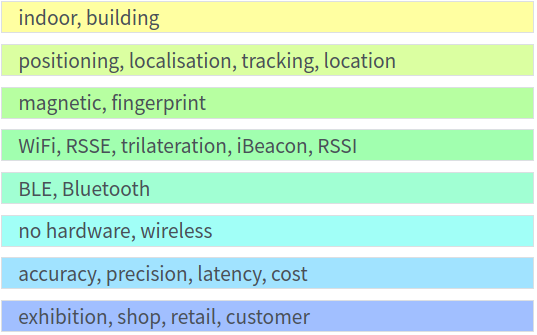
\includegraphics[width=0.48\textwidth]{img/patents/color.png}
    \caption{.}
    \label{fig:Patent-highlighting}
\end{figure}

Patents search highlighting categories which were used to build the classifier.

\begin{figure}[h]
    \centering
    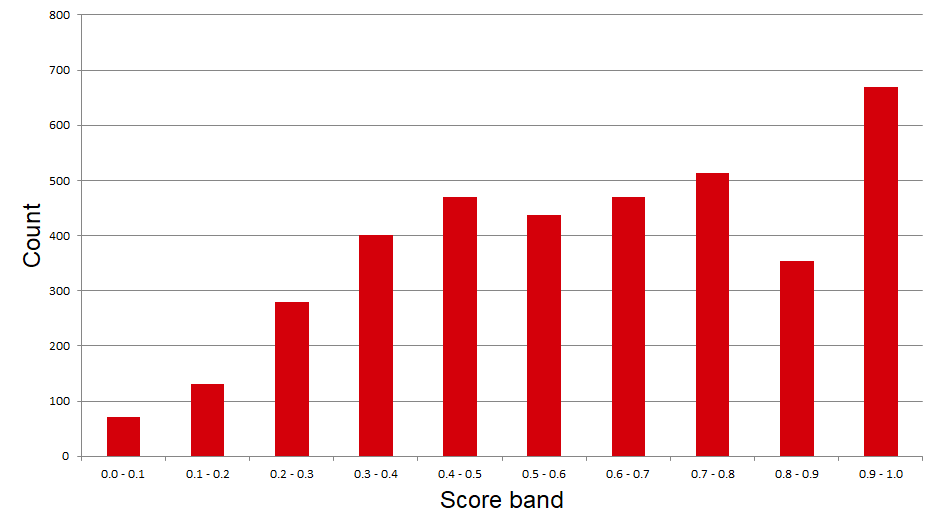
\includegraphics[width=0.48\textwidth]{img/patents/score.png}
    \caption{Patents result score of final report.}
    \label{fig:Patent-score}
\end{figure}

Result score shown on the \ref{fig:Patent-score} show how patents fit the classifier.


Second part is focused on building a model of a product and optimizing it for several criteria.
We focus on the system architecture of indoor positioning solutions. The system architecture provided by the Indoor Location Alliance is used as the main reference. Next we use the data from the Microsoft indoor positioning competition. This is a valuable data, because it provides data about development of indoor positioning technologies and their performance. Data of teams who are competing in the same conditions are perfect for benchmarking. Having the data of benchmarking, we may define technology complexity in real numbers and use it when builing the strategy.
% For this we use OPM (object process management) models and OPCAT simulator, UML diagrams, risk matrice and code based models containing figure of merits interconnections. We don't do optimization of a product here, just list possible options with [] curves.

Third we do a financial valuation. We collect all data about product, market, marketing channells and model of sales together.
Having existing business model which is outside of the scope of this paper, we may identify numbers of sales and revenues.
We use the costs and amount of investments we need to complete this project.
We tune the finantial model to obtain the positive NPV. To be coherent with the product figures of merits, we also adjust values of the model to receive a non-dominated product on the market.

Next we do value at risk analysis. With the value at risk gain curve, we check different financial models.
 % comparing to the Pareto frontier.

After all procedures we come up with bunch of strategies from where we can choose one. Again, we can't make decisions based on this models, but we can check strategies performance and for different technical decisions.

\subsection{Intellectual Property, Publications}
